% ===== Block 2: Kubernetes Core (slides 37-94) =====
\sectionframe{Kubernetes}

% --- What is Kubernetes? (band + logos + bubble) ---
\begin{frame}{What is Kubernetes?}
  \orangeband{Kubernetes is an open-source system for automating deployment,
  scaling, and management of containerized applications.}
  \vfill
  \begin{columns}[c]
    \column{0.26\textwidth}
      \centering
\includegraphics[height=2.8cm]{assets/k8s-logo.png}
    \column{0.46\textwidth}
      \centering
      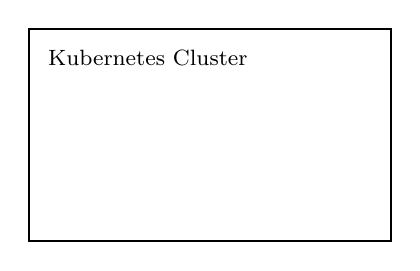
\begin{tikzpicture}
        \draw[thick] (0,0) rectangle (4.6,2.7);
        \node[anchor=north west, font=\footnotesize] at (0.12,2.55) {Kubernetes Cluster};
      \end{tikzpicture}
    \column{0.26\textwidth}
      \centering
\includegraphics[height=2.4cm]{assets/cncf-logo.png}
  \end{columns}
  \vfill
  \begin{tikzpicture}[remember picture, overlay]
    \bubble{\pg{4.9cm}{-7.2cm}}{\pg{3.2cm}{-6.0cm}}{Kubernetes originates from Greek, meaning ``helmsman'' or ``pilot''}
  \end{tikzpicture}
\end{frame}

% --- Kubernetes Management: Rancher ---
\begin{frame}{Kubernetes Management: \wsClusterPlatform}
  \begin{columns}[c]
    \column{0.62\textwidth}
      \begin{itemize}
        \item What is \wsClusterPlatform?
          \begin{itemize}
            \item Kubernetes {\color{wsorange}\textbf{Orchestration Platform}}
            \item Multi-Cluster Management
          \end{itemize}
        \item Why \wsClusterPlatform?
          \begin{itemize}
            \item UI to interact with clusters
            \item {\color{wsorange}\textbf{Manage access}} clusters
            \item {\color{wsorange}\textbf{Manage projects}}
          \end{itemize}
      \end{itemize}
    \column{0.34\textwidth}
      \centering
\includegraphics[width=0.9\linewidth]{assets/rancher-logo.pdf}
  \end{columns}
\end{frame}

% --- Warning ---
\begin{frame}{Warning!}
  \begin{itemize}
    \item Everything created in the workshop \wsClusterPlatform{} project will be deleted!
    \item You may use the cluster for your project at the host institution
      \begin{itemize}
        \item Practical-course teams can request Kubernetes access
        \item Every DevOps team gets a \wsClusterPlatform{} project automatically
      \end{itemize}
    \item The cluster has a fair use policy!
      \begin{itemize}
        \item Only reserve what you really need
        \item Make sure your code / deployment is not vulnerable
        \item Projects that misbehave are removed without notice
      \end{itemize}
  \end{itemize}
\end{frame}

% --- Exercise: Get access to Rancher ---
\begin{frame}{Exercise: Get Access To \wsClusterPlatform}
  \vspace{1cm}
  \begin{enumerate}
    \item Task 1: open \underline{\wsClusterURL}
    \item Task 2: log in with \wsAccountWording
    \item Task 3: access the Student Cluster
  \end{enumerate}
\end{frame}

% --- Exercise: kubectl ---
\begin{frame}{Exercise: kubectl}
  \begin{enumerate}
    \item Task 1: download the \texttt{kubeconfig}
    \item Task 2: put the \texttt{kubeconfig} into \texttt{\textasciitilde/.kube/config}
    \item Task 3: ensure the connection works: \texttt{kubectl cluster-info}
  \end{enumerate}
  \bigskip
  If you already have something in there, create a backup of the file first.
\end{frame}

\breakframe

% --- Kubernetes API and API objects ---
\begin{frame}{Kubernetes API and API objects}
  \begin{itemize}
    \item Namespace
    \item Pod
    \item Workloads
      \begin{itemize}\item (ReplicaSet) \item Deployment\end{itemize}
    \item Service
    \item Ingress
  \end{itemize}
\end{frame}

% ===== Namespace =====
\objframe{0.30}{0.88}{0.55}{1.0}   % Namespace

\begin{frame}[fragile]{Namespaces}
  \begin{columns}[c]
    \column{0.5\textwidth}
      \begin{itemize}
        \item \textbf{Isolate} groups of \textbf{resources}
        \item Encapsulate / \textbf{scope names}
          \begin{itemize}\item Names of resources within a Namespace have to be unique\end{itemize}
        \item \textbf{Access control}
        \item Resource quotas
      \end{itemize}
    \column{0.48\textwidth}
      \yamlfile{../slide-examples/10-kubernetes-namespace/namespace.yml}
  \end{columns}
\end{frame}

\begin{frame}[fragile]{Get to know the cluster}
  \begin{itemize}
    \item Create a namespace (important step to work with the \wsClusterPlatform{} cluster)
      \begin{itemize}
        \item Open \wsClusterPlatform{} and navigate to the respective cluster
        \item Select Cluster $>$ Projects/Namespaces
        \item Click the ``Create Namespace'' button in the respective project
      \end{itemize}
    \item See what is running in a specific namespace:
  \end{itemize}
  \begin{termbox}
\begin{lstlisting}[style=wstermstyle]
kubectl -n <namespace> get all
\end{lstlisting}
  \end{termbox}
\end{frame}

% ===== Pod =====
\objframe{0.38}{0.48}{0.62}{0.60}  % Pod

\begin{frame}{Pods}
  \begin{columns}[c]
    \column{0.56\textwidth}
      \begin{itemize}
        \item {\color{wsorange}\textbf{Smallest deployable computing unit}} in Kubernetes
        \item Group of {\color{wsorange}\textbf{one or more containers}}
        \item Ephemeral nature
          \begin{itemize}\item ``Designed to be destroyed''\end{itemize}
        \item Containers within a Pod {\color{wsorange}\textbf{share}}
          \begin{itemize}\item Storage \item Network (IP address)\end{itemize}
        \item It is uncommon to work with \texttt{Pods} directly
      \end{itemize}
    \column{0.4\textwidth}
      \centering
      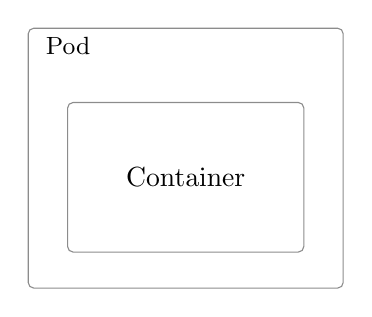
\begin{tikzpicture}
        \node[draw=black!45, rounded corners=2pt, minimum width=4cm, minimum height=3.3cm, anchor=north] (pod) at (0,0) {};
        \node[anchor=north west, font=\small] at (pod.north west) {\ Pod};
        \node[draw=black!45, rounded corners=2pt, minimum width=3cm, minimum height=1.9cm] at (0,-1.9) {Container};
      \end{tikzpicture}
      \par\smallskip
      \colorbox{wsyellow}{\bfseries\small Mostly one container per pod}
  \end{columns}
\end{frame}

\begin{frame}[fragile]{Pods: manifest}
  \begin{columns}[c]
    \column{0.5\textwidth}
      \begin{itemize}
        \item {\color{wsorange}\textbf{Smallest deployable computing unit}} in Kubernetes
        \item Group of {\color{wsorange}\textbf{one or more containers}}
        \item Ephemeral nature
        \item Containers within a Pod {\color{wsorange}\textbf{share}} storage and network
        \item It is uncommon to work with \texttt{Pods} directly
      \end{itemize}
    \column{0.48\textwidth}
      \yamlfile{../slide-examples/11-kubernetes-pod/pod.yml}
  \end{columns}
\end{frame}

% --- Pods: manifest explained (field bubbles) ---
\begin{frame}[fragile]{Pods: manifest explained}
  \begin{columns}[T]
    \column{0.5\textwidth}
      \begin{yamlbox}
\begin{lstlisting}[style=wsyamlstyle, basicstyle=\ttfamily\scriptsize]
apiVersion: v1
kind: Pod
metadata:
  (*\tikzmark{pn}*)name: app1
  namespace: my-namespace
  (*\tikzmark{pl}*)labels:
    exampleLabel: my-app1
spec:
  (*\tikzmark{pc}*)containers:
    (*\tikzmark{pi}*)- name: app1
      image: nginxdemos/hello
      (*\tikzmark{pp}*)ports:
        - containerPort: 80
\end{lstlisting}
      \end{yamlbox}
    \column{0.48\textwidth}
  \end{columns}
  \begin{tikzpicture}[remember picture, overlay]
    \bubbleat{\pg{9.5cm}{-2.2cm}}{pn}{Name and Namespace of the Pod}
    \bubbleat{\pg{9.5cm}{-3.3cm}}{pl}{Labels to select the Pod later on}
    \bubbleat{\pg{9.5cm}{-4.4cm}}{pc}{List of containers in the Pod}
    \bubbleat{\pg{9.5cm}{-5.5cm}}{pi}{Name and image of the container}
    \bubbleat{\pg{9.5cm}{-6.6cm}}{pp}{List of ports to the container}
  \end{tikzpicture}
\end{frame}

\begin{frame}[fragile]{Get to know the cluster}
  \begin{itemize}\item Deploy a manifest (``stating your wishlist''):\end{itemize}
  \begin{termbox}
\begin{lstlisting}[style=wstermstyle]
kubectl apply -f example.yaml
\end{lstlisting}
  \end{termbox}
  \begin{itemize}\item Delete all resources in the manifest:\end{itemize}
  \begin{termbox}
\begin{lstlisting}[style=wstermstyle]
kubectl delete -f example.yaml
\end{lstlisting}
  \end{termbox}
\end{frame}

\begin{frame}[fragile]{Debugging in Kubernetes}
  \begin{itemize}\item Get a Kubernetes resource:\end{itemize}
  \begin{termbox}
\begin{lstlisting}[style=wstermstyle]
kubectl [-n namespace] get pod
\end{lstlisting}
  \end{termbox}
  \begin{itemize}\item Get details about a Kubernetes resource:\end{itemize}
  \begin{termbox}
\begin{lstlisting}[style=wstermstyle]
kubectl [-n namespace] describe pod <name>
\end{lstlisting}
  \end{termbox}
\end{frame}

% ===== Deployment =====
\objframe{0.38}{0.24}{0.63}{0.36}  % Deployment

\begin{frame}[fragile]{Deployments}
  \begin{columns}[c]
    \column{0.5\textwidth}
      \begin{itemize}
        \item {\color{wsorange}\textbf{Declarative control group}} for \texttt{Pods} and \texttt{ReplicaSets}
        \item Manages {\color{wsorange}\textbf{application scaling}}
        \item Manages {\color{wsorange}\textbf{rollout}} and {\color{wsorange}\textbf{rollback}}
        \item \texttt{LabelSelector} based
      \end{itemize}
    \column{0.48\textwidth}
      \yamlfile{../slide-examples/12-kubernetes-deployment/deployment.yml}
  \end{columns}
\end{frame}

\begin{frame}[fragile]{Deployments: manifest explained}
  \begin{columns}[T]
    \column{0.5\textwidth}
      \begin{yamlbox}
\begin{lstlisting}[style=wsyamlstyle, basicstyle=\ttfamily\scriptsize]
apiVersion: apps/v1
kind: Deployment
metadata:
  (*\tikzmark{dn}*)name: app1-deployment
  namespace: my-namespace
spec:
  (*\tikzmark{dr}*)replicas: 1
  (*\tikzmark{ds}*)selector:
    matchLabels:
      app: app1-selector
  (*\tikzmark{dt}*)template:
    metadata:
      (*\tikzmark{dl}*)labels:
        app: app1-selector
    spec:
      (*\tikzmark{dc}*)containers:
        - name: app1-container
          image: nginx:stable
\end{lstlisting}
      \end{yamlbox}
    \column{0.48\textwidth}
  \end{columns}
  \begin{tikzpicture}[remember picture, overlay]
    \bubbleat[text width=3.8cm]{\pg{9.7cm}{-1.9cm}}{dn}{Name and Namespace}
    \bubbleat[text width=3.8cm]{\pg{9.7cm}{-2.9cm}}{dr}{Number of Pods to create}
    \bubbleat[text width=3.8cm]{\pg{9.7cm}{-3.9cm}}{ds}{Pod selector}
    \bubbleat[text width=3.8cm]{\pg{9.7cm}{-4.9cm}}{dt}{Template for Pods}
    \bubbleat[text width=3.8cm]{\pg{9.7cm}{-5.9cm}}{dl}{Labels spawned Pods receive}
    \bubbleat[text width=3.8cm]{\pg{9.7cm}{-6.9cm}}{dc}{Name and image of containers}
  \end{tikzpicture}
\end{frame}

% ===== LabelSelector =====
\objframe{0.78}{0.60}{1.0}{0.75}   % LabelSelector

\begin{frame}[fragile]{Interacting with Deployments}
  \begin{termbox}
\begin{lstlisting}[style=wstermstyle, basicstyle=\ttfamily\scriptsize\color{wsgreen}]
kubectl apply -f deployment.yaml          # deploy
kubectl describe deployment <name>        # inspect
kubectl logs deployment/<name>            # logs
kubectl scale deployment <name> --replicas=3
kubectl rollout undo deployment <name>    # revert
\end{lstlisting}
  \end{termbox}
\end{frame}

\begin{frame}{Exercise: Deployment for the reservation system}
  \begin{enumerate}
    \item \sout{Task 1: configure the cluster to pull from a private registry} (see appendix)
    \item Task 2: create a deployment manifest for the reservation system
  \end{enumerate}
  \bigskip You can use the templates in your repo as a starting point.
\end{frame}

\begin{frame}{Task 2: Create reservation deployment}
  \centering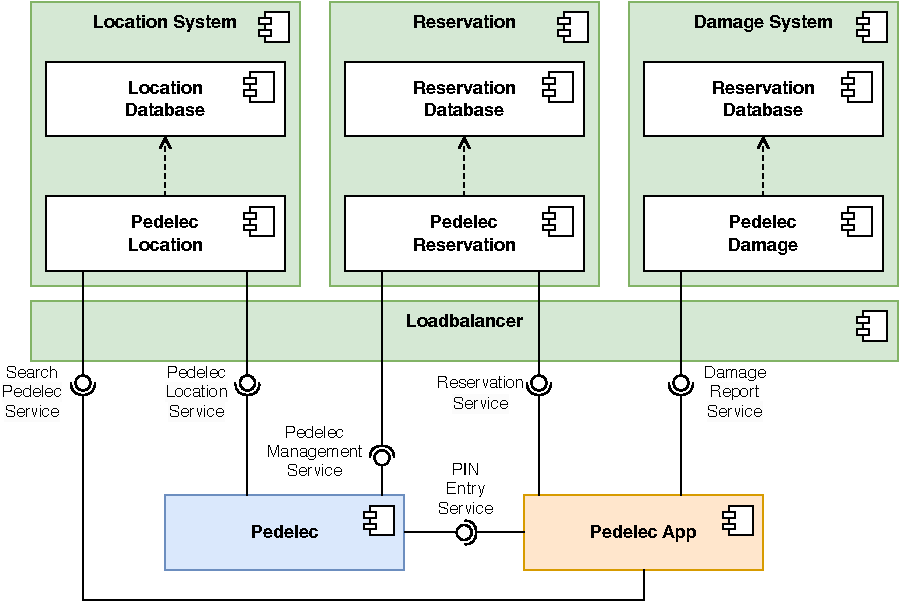
\includegraphics[height=0.72\paperheight]{assets/dia-pedelec-ssd.pdf}
\end{frame}

\begin{frame}[fragile]{Task 2: reservation deployment manifest}
  \begin{columns}[c]
    \column{0.52\textwidth}
      \yamlfile{../slide-examples/13-kubernetes-deployment-reservation/reservation-deployment.yml}
    \column{0.44\textwidth}
      Image: \imgref{reservation}
      \begin{itemize}
        \item Remember to update the namespace to your own!
        \item Resource limits are omitted here; you will see them in the demo.
      \end{itemize}
  \end{columns}
\end{frame}

\breakframe

% ===== Service =====
\begin{frame}{We have a problem now\ldots}
  \begin{itemize}
    \item We learned that
      \begin{itemize}
        \item Pods are ephemeral
        \item Get a new IP address on every schedule
        \item Are scattered over all Kubernetes nodes
      \end{itemize}
    \item How do we find them then?
      \begin{itemize}\item $\rightarrow$ Services\end{itemize}
  \end{itemize}
\end{frame}

\objframe{0.38}{0.12}{0.62}{0.24}  % Service

% ISO/OSI with "Service lives here" bubble at Layer 4
\begin{frame}{ISO/OSI model}
  \centering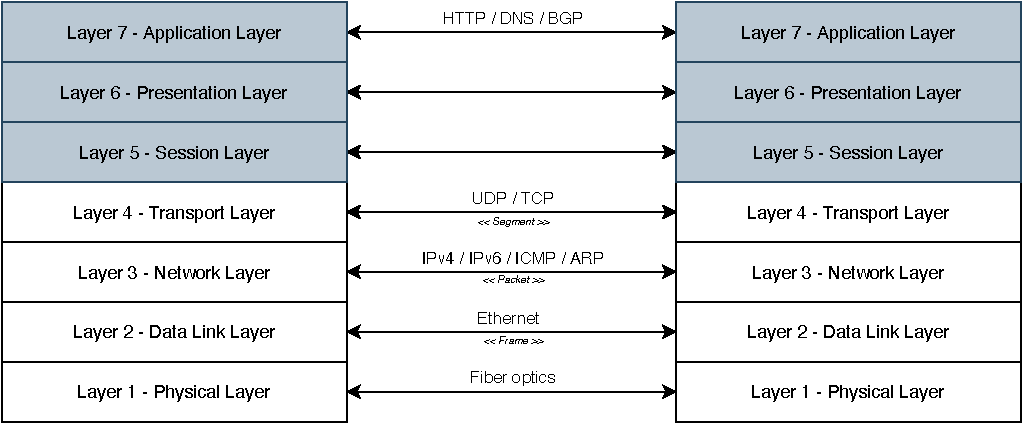
\includegraphics[width=\textwidth,height=0.66\paperheight,keepaspectratio]{assets/dia-osi.pdf}
  \begin{tikzpicture}[remember picture, overlay]
    \bubble{\pg{10.6cm}{-5.0cm}}{\pg{8.2cm}{-4.7cm}}{The Service lives here (Layer 4)}
  \end{tikzpicture}
\end{frame}

\begin{frame}[fragile]{Services}
  \begin{columns}[c]
    \column{0.5\textwidth}
      \begin{itemize}
        \item Abstraction layer to expose a set of \texttt{Pods}
        \item Manages {\color{wsorange}\textbf{service discovery}}
        \item Manages {\color{wsorange}\textbf{load balancing}} to Pods
        \item IP addressable
        \item \texttt{LabelSelector} based
      \end{itemize}
    \column{0.48\textwidth}
      \yamlfile{../slide-examples/14-kubernetes-service/service.yml}
  \end{columns}
\end{frame}

\begin{frame}[fragile]{Services: manifest explained}
  \begin{columns}[T]
    \column{0.5\textwidth}
      \begin{yamlbox}
\begin{lstlisting}[style=wsyamlstyle, basicstyle=\ttfamily\scriptsize]
apiVersion: v1
kind: Service
metadata:
  (*\tikzmark{sn}*)name: app1-service
  namespace: my-namespace
spec:
  (*\tikzmark{ss}*)selector:
    app: app1-selector
  ports:
    (*\tikzmark{sp}*)- port: 80
      (*\tikzmark{st}*)targetPort: app1-port
\end{lstlisting}
      \end{yamlbox}
    \column{0.48\textwidth}
  \end{columns}
  \begin{tikzpicture}[remember picture, overlay]
    \bubbleat{\pg{9.5cm}{-2.4cm}}{sn}{Name and Namespace of the Service}
    \bubbleat{\pg{9.5cm}{-3.6cm}}{ss}{Pod selector: who can I send traffic to}
    \bubbleat{\pg{9.5cm}{-4.8cm}}{sp}{Port the Service exposes}
    \bubbleat{\pg{9.5cm}{-6.0cm}}{st}{Port the Service connects to}
  \end{tikzpicture}
\end{frame}

% Service topology build-ups (TikZ)
\begin{frame}{Services}
  \textbf{Kubernetes Cluster}
  \vfill\centering
  \begin{tikzpicture}[node distance=6mm]
    \node[tpod] at (0,1) {\scriptsize$\ll$Pod$\gg$\\Reservation};
    \node[tpod] at (2,2) {\scriptsize$\ll$Pod$\gg$\\Damage};
    \node[tpod] at (5,1.4) {\scriptsize$\ll$Pod$\gg$\\Reservation};
    \node[tpod] at (1,-0.6) {\scriptsize$\ll$Pod$\gg$\\Reservation};
    \node[tpod] at (3,-0.4) {\scriptsize$\ll$Pod$\gg$\\Damage};
    \node[tpod] at (4.4,-0.2) {\scriptsize$\ll$Pod$\gg$\\Reservation};
  \end{tikzpicture}\vfill
\end{frame}

\begin{frame}{Services}
  \textbf{Kubernetes Cluster}
  \vfill\centering
  \begin{tikzpicture}
    \node[tsvc] (svc) at (2.2,2.2) {\scriptsize$\ll$Service$\gg$\\Reservation};
    \foreach \x/\n in {0/1,1.5/2,3/3,4.5/4}
      \node[tpod] (p\n) at (\x,0) {\scriptsize$\ll$Pod$\gg$\\Reservation};
    \foreach \n in {1,2,3,4} \draw (svc) -- (p\n);
  \end{tikzpicture}\vfill
  \begin{center}\colorbox{wsyellow}{\bfseries\small Single point of entry to all selected (``backing'') Pods}\end{center}
\end{frame}

\begin{frame}{Exercise: Service for the reservation system}
  \begin{enumerate}
    \item Task 1: create a Service manifest for the reservation system
    \item Task 2: get the Service details using \texttt{kubectl}
  \end{enumerate}
\end{frame}

\begin{frame}[fragile]{Task 1: reservation service manifest}
  \begin{columns}[c]
    \column{0.52\textwidth}
      \yamlfile{../slide-examples/15-kubernetes-service-reservation/reservation-service.yml}
    \column{0.44\textwidth}
      \colorbox{wsyellow}{\parbox{\linewidth}{\bfseries\small We use the same label to select the matching Pods}}
  \end{columns}
\end{frame}

% ===== Ingress =====
\objframe{0.40}{0.0}{0.63}{0.12}   % Ingress

\begin{frame}{Kubernetes Ingresses}
  \orangeband{An Ingress is a Kubernetes API object that manages external access
  to services in a cluster, typically via HTTP/HTTPS.}
  \begin{itemize}
    \item \textbf{Central entry point} for multiple services (reverse proxy)
    \item Clean URL routing (e.g., \texttt{/api}, \texttt{/admin})
    \item \textbf{TLS termination} (HTTPS)
    \item Path-based and host-based routing
    \item An ingress needs to be implemented by an \textbf{IngressController}
  \end{itemize}
\end{frame}

\begin{frame}{Ingress: path-based fan-out}
  \textbf{Kubernetes Cluster}\hfill\texttt{\wsIngressBase}
  \vfill\centering
  \begin{tikzpicture}
    \node[ting] (ing) at (2.2,2.4) {\scriptsize$\ll$Ingress$\gg$\\Pedelec};
    \node[tsvc] (l) at (0,0) {\scriptsize$\ll$Service$\gg$\\Location};
    \node[tsvc] (r) at (2.2,0) {\scriptsize$\ll$Service$\gg$\\Reservation};
    \node[tsvc] (d) at (4.4,0) {\scriptsize$\ll$Service$\gg$\\Damage};
    \draw (ing) -- node[above left, font=\tiny]{\texttt{/location}} (l);
    \draw (ing) -- node[right, font=\tiny]{\texttt{/reservation}} (r);
    \draw (ing) -- node[above right, font=\tiny]{\texttt{/damage}} (d);
  \end{tikzpicture}\vfill
\end{frame}

\begin{frame}[fragile]{Ingress}
  \begin{columns}[c]
    \column{0.5\textwidth}
      \begin{itemize}
        \item \textbf{Exposes} Services outside the cluster via \textbf{HTTP/HTTPS}
        \item Backed by an IngressController
        \item Acts like a ``Reverse Proxy''
      \end{itemize}
    \column{0.48\textwidth}
      \yamlfile{../slide-examples/16-kubernetes-ingress/ingress.yml}
  \end{columns}
\end{frame}

\begin{frame}[fragile]{Ingress: manifest explained}
  \begin{columns}[T]
    \column{0.52\textwidth}
      \begin{yamlbox}
\begin{lstlisting}[style=wsyamlstyle, basicstyle=\ttfamily\tiny]
(*\tikzmark{in}*)apiVersion: networking.k8s.io/v1
kind: Ingress
metadata:
  (*\tikzmark{im}*)name: app1-ingress
  namespace: my-namespace
  (*\tikzmark{ia}*)annotations:
    nginx.ingress.kubernetes.io/rewrite-target: /
spec:
  rules:
    (*\tikzmark{ih}*)- host: example.com
      http:
        paths:
          (*\tikzmark{ip}*)- path: /
            pathType: Prefix
            (*\tikzmark{ib}*)backend:
              service:
                name: app1-service
\end{lstlisting}
      \end{yamlbox}
    \column{0.46\textwidth}
  \end{columns}
  \begin{tikzpicture}[remember picture, overlay]
    \bubbleat[text width=3.9cm]{\pg{9.9cm}{-1.7cm}}{in}{Notice the different apiVersion}
    \bubbleat[text width=3.9cm]{\pg{9.9cm}{-2.7cm}}{im}{Name and Namespace}
    \bubbleat[text width=3.9cm]{\pg{9.9cm}{-3.7cm}}{ia}{Arbitrary non-identifying metadata}
    \bubbleat[text width=3.9cm]{\pg{9.9cm}{-4.7cm}}{ih}{Hostname the ingress listens for}
    \bubbleat[text width=3.9cm]{\pg{9.9cm}{-5.7cm}}{ip}{Path the ingress routes}
    \bubbleat[text width=3.9cm]{\pg{9.9cm}{-6.7cm}}{ib}{Service and Port of the backing Service}
  \end{tikzpicture}
\end{frame}

\begin{frame}{Exercise: Ingress for the Pedelec server}
  \begin{enumerate}
    \item Task 1: single Ingress deployment
    \item Task 2: test the endpoints with Bruno
    \item Task 3: add remaining endpoints to the ingress
  \end{enumerate}
\end{frame}

\begin{frame}[fragile]{Important notes}
  \begin{columns}[T]
    \column{0.5\textwidth}
      \begin{itemize}
        \item You can \textbf{only use} hosts under \texttt{*.\wsIngressBase} by default
        \item The backing pod must \textbf{expect the correct route}
        \item \textbf{Ingress configurations} are heavily based on annotations
          \begin{itemize}
            \item Request a \textbf{TLS certificate} via an annotation
            \item Test with staging first ;)
          \end{itemize}
      \end{itemize}
      \smallskip Let's Encrypt has strict rate-limiting policies.
    \column{0.48\textwidth}
      \begin{yamlbox}
\begin{lstlisting}[style=wsyamlstyle, basicstyle=\ttfamily\scriptsize]
annotations:
  cert-manager.io/cluster-issuer:
    letsencrypt-staging
spec:
  tls:
    - hosts:
        - pedelec.com
      secretName: reservation-tls
  rules:
    - host: pedelec.com
\end{lstlisting}
      \end{yamlbox}
  \end{columns}
\end{frame}

\begin{frame}{From Compose to Kubernetes}
  \begin{itemize}
    \item Keep in mind: \textbf{this mapping is not general advice but sufficient for this example!}
  \end{itemize}
  \vfill\centering
  \begin{tabular}{c c c}
    \textbf{Docker World} & & \textbf{Kubernetes World}\\[2pt]
    Service & $\rightarrow$ & Deployment\\
    Expose  & $\rightarrow$ & Service\\
    Port    & $\rightarrow$ & Service / Ingress\\
  \end{tabular}
  \vfill
  \begin{center}\colorbox{wsnavy}{\color{white}\bfseries\small Docker and Kubernetes use the word ``Service'' to describe different things!}\end{center}
\end{frame}
